% Created 2016-06-18 Sa 23:26
\documentclass{beamer}
\usepackage[utf8]{inputenc}
\usepackage[T1]{fontenc}
\usepackage{fixltx2e}
\usepackage{graphicx}
\usepackage{grffile}
\usepackage{longtable}
\usepackage{wrapfig}
\usepackage{rotating}
\usepackage[normalem]{ulem}
\usepackage{amsmath}
\usepackage{textcomp}
\usepackage{amssymb}
\usepackage{capt-of}
\usepackage{hyperref}
\usepackage{listings}
\usetheme{default}
\author{Sebastian Ullrich}
\date{OPLSS 2016}
\title{Electrolysis}
\subtitle{Verifying Rust Programs via Functional Purification\\[5mm]

\includegraphics[scale=1.4]{../logo}\\[-3mm]}
\institute[]{Karlsruhe Institute of Technology, advisor Gregor Snelting \\[1mm]
Carnegie Mellon University, advisor Jeremy Avigad}
\hypersetup{
 pdfauthor={Sebastian Ullrich},
 pdftitle={Electrolysis - Verifying Rust Programs via Functional Purification},
 pdflang={English}}
\begin{document}

\maketitle

%\begin{frame}{Outline}
%\tableofcontents
%\end{frame}

\section{Why Rust}

\begin{frame}{Why Rust? (What is Rust?)}
  Rust is a new systems programming language sponsored by Mozilla Research
  \begin{itemize}
    \item multi-paradigm with an ML-like syntax
    \item pursues ``the trifecta: safety, concurrency, and speed''
      \begin{itemize}
        \item \alert{speed} through zero-cost abstractions and manual memory management
        \item \alert{memory safety} through tracking reference lifetimes in the type system
        \item \alert{safe concurrency} through forbidding shared mutable references
      \end{itemize}
  \end{itemize}
  \uncover<2>{
    \begin{center}
      
\includegraphics[height=3cm]{rustacean-orig-happy}
    \end{center}
  }
\end{frame}

\begin{frame}[fragile]{Why Rust: Because It's Almost Pure Already}
  \begin{itemize}
    \item turn destructive updates into functional ones
      \begin{columns}
        \column{0.25\textwidth}
        \color{gray}
        \begin{verbatim}
p.x += 1;
        \end{verbatim}
        \column{0.5\textwidth}
        \begin{verbatim}
let p = Point { x = p.x + 1, ..p };
        \end{verbatim}
      \end{columns}
    \item references: save value instead of pointer, write back at end of lifetime
      \begin{columns}
        \column{0.25\textwidth}
        \color{gray}
        \begin{verbatim}
let x = f(&mut p);
        \end{verbatim}
        \column{0.5\textwidth}
        \begin{verbatim}
let (x, p) = f(p);
        \end{verbatim}
      \end{columns}
  \end{itemize}
\end{frame}

\section{Simple Verification via Purification}

\setbeamercovered{transparent}
\begin{frame}[t]{Simple Verification via Purification}
  \begin{enumerate}
    \item \uncover<1>{make Rust program purely functional}
    \item transpile it into expression language of a theorem prover (Lean)
      \only<2>{
        \begin{itemize}
          \item run \texttt{rustc} up to CFG generation
          \item sort definitions topologically by dependencies
          \item extract loops from CFG and put them into loop combinator
          \item resolve static/dynamic trait calls
        \end{itemize}

        \hfill

        Things Rust fortunately does not have:
        \begin{itemize}
          \item exceptions
          \item subtyping
        \end{itemize}
      }
    \item \uncover<1>{prove correctness of the Lean definition}
  \end{enumerate}
\end{frame}

\section{Verifying \texttt{std::[T]::binary\_search}}

\begin{frame}{Verifying \texttt{std::[T]::binary\_search}: Input}
  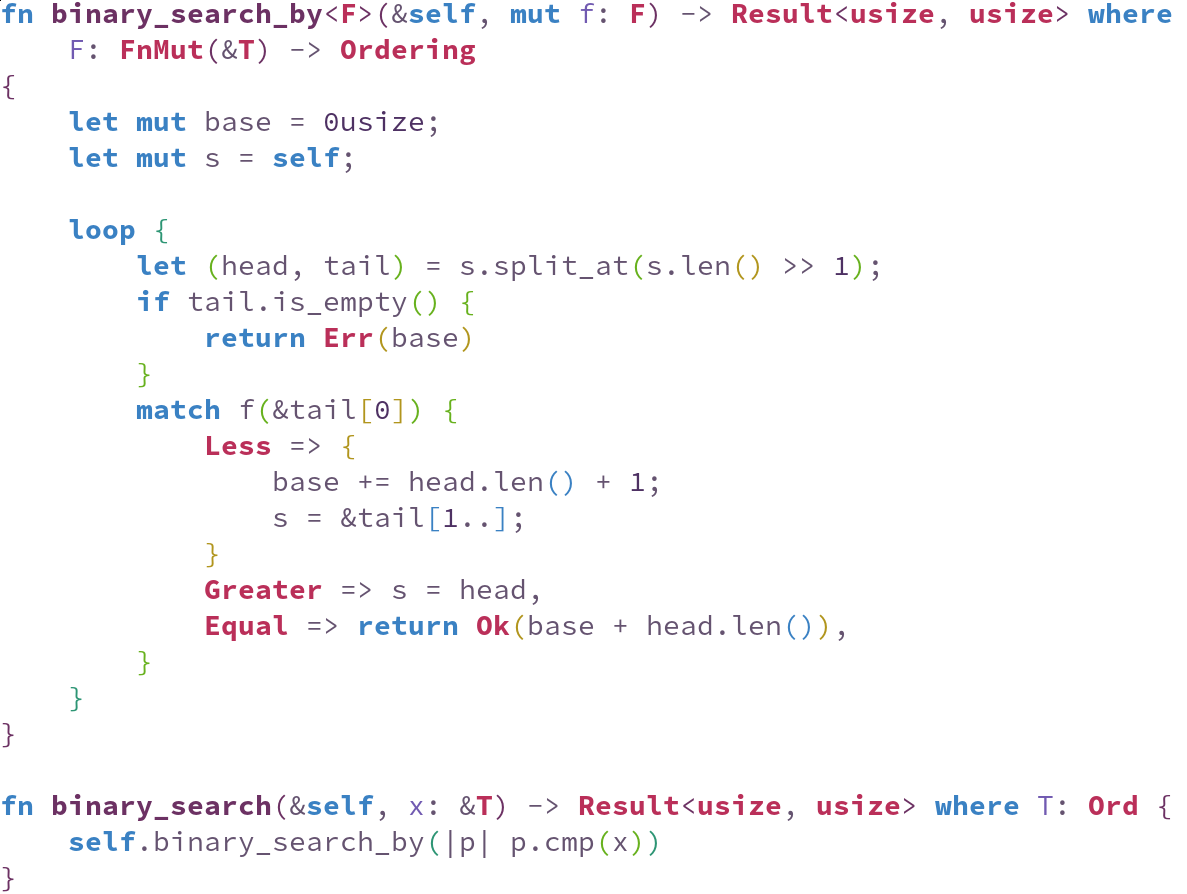
\includegraphics[height=0.5\textheight]{binary_search}
  \begin{itemize}
    \item high-level implementation working with subslices instead of explicit indicing
    \item transitively uses
      \begin{itemize}
        \item[5] traits
        \item[6] structs and enums
        \item[7] functions
      \end{itemize}
  \end{itemize}
\end{frame}

\begin{frame}{Verifying \texttt{std::[T]::binary\_search}: Output}
  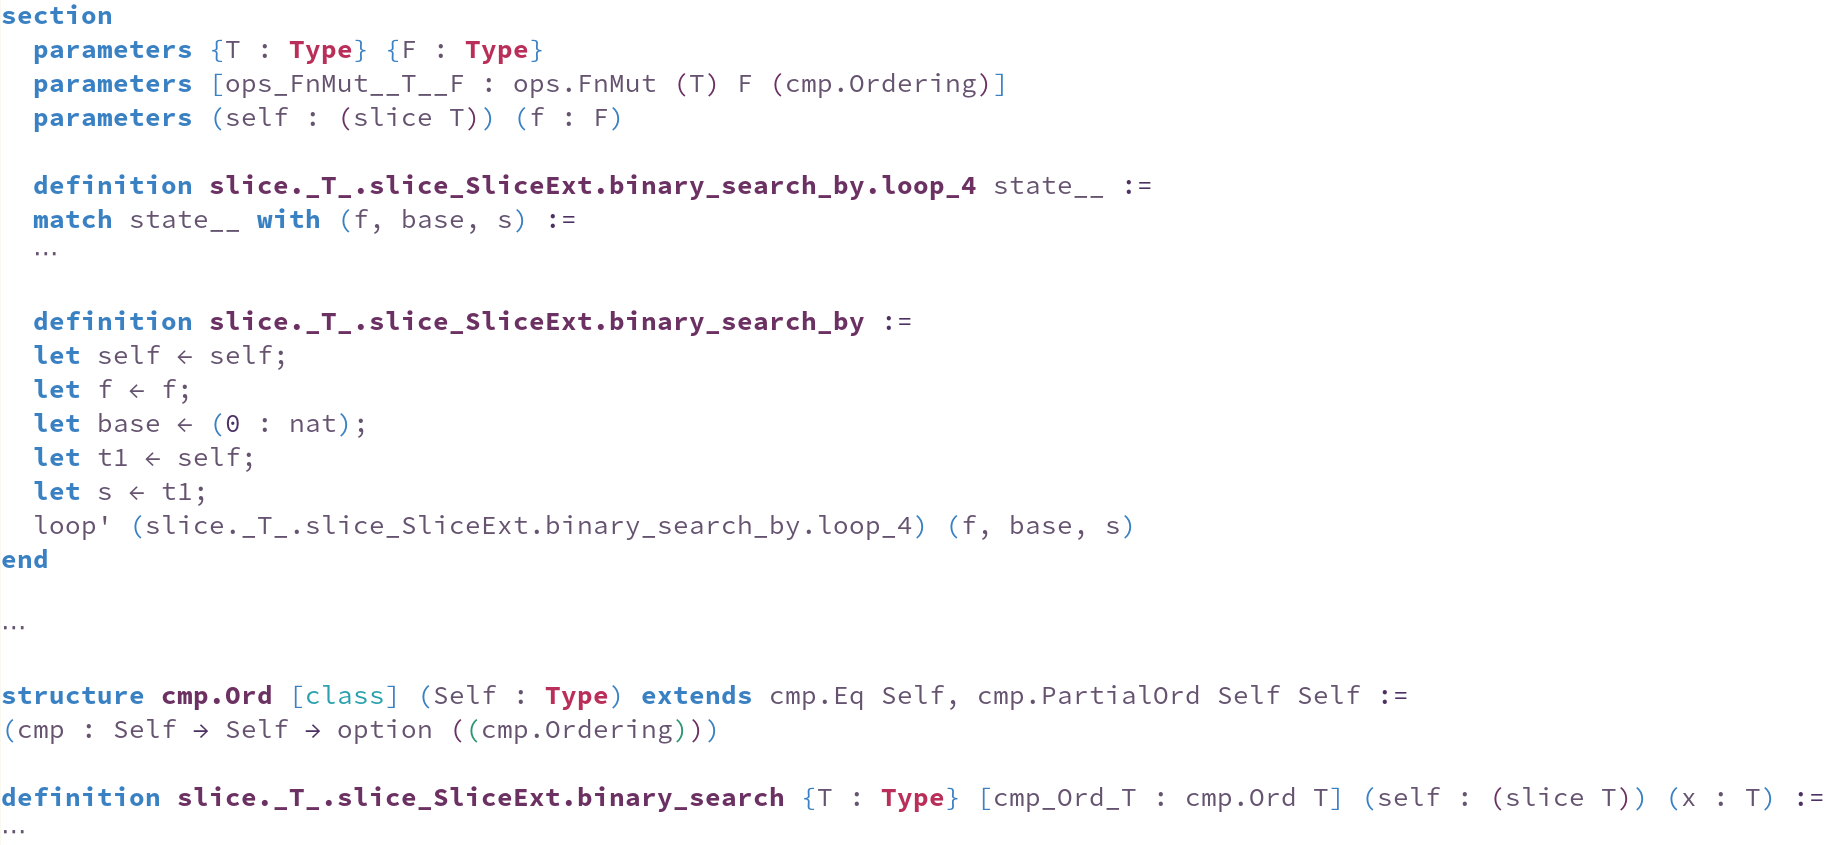
\includegraphics[width=\textwidth]{generated}
\end{frame}

\begin{frame}{Verifying \texttt{std::[T]::binary\_search}: Proof}
  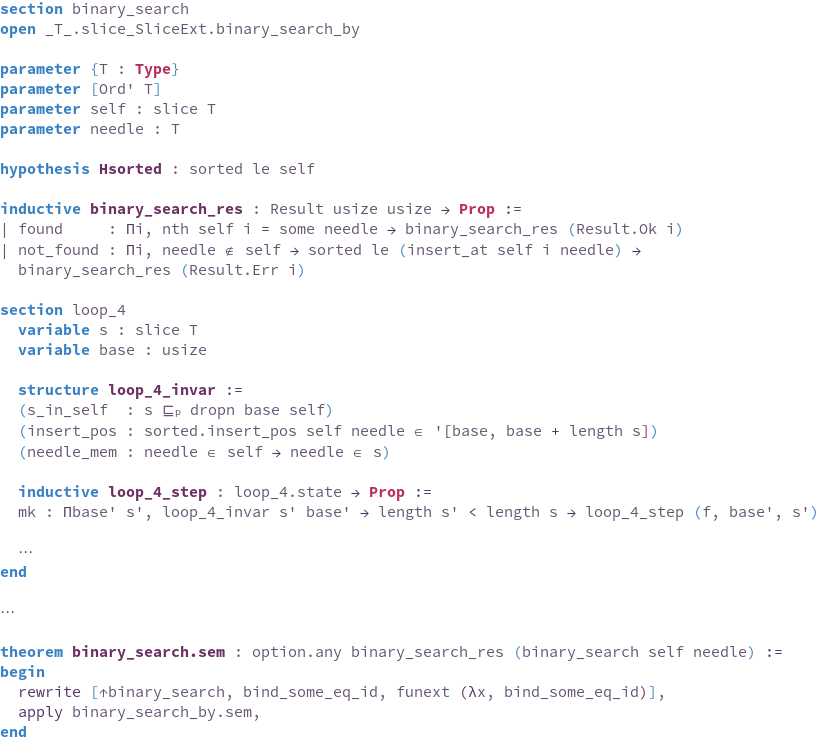
\includegraphics[height=0.8\textheight,trim=0 0 0 20mm, clip]{proof}
\end{frame}

\section{Conclusion and Future Work}

\begin{frame}{Conclusion and Future Work}
  \begin{itemize}
    \item a tool for verifying real-world Rust code
    \item correctness proof of a central stdlib algorithm

    \hfill

    \item next step: find a new algorithm to verify!
    \item possible enhancement: different monad stacks for e.g.\ complexity analysis, global side effects, \dots
    \item maybe allow some restricted forms of unsafe code
  \end{itemize}

  \hfill

  \begin{center}
    \large\url{github.com/Kha/electrolysis}
  \end{center}
\end{frame}

\end{document}
